\documentclass[10pt]{article}
\usepackage[utf8]{inputenc}
\usepackage[T1]{fontenc}
\usepackage{amsmath}
\usepackage{amsfonts}
\usepackage{amssymb}
\usepackage[version=4]{mhchem}
\usepackage{stmaryrd}
\usepackage{graphicx}
\usepackage[export]{adjustbox}
\graphicspath{ {./images/} }

\begin{document}
\begin{enumerate}
  \item Find $B C$ in the triangle shown below. Round your answer to the nearest thousandth.
  \item Find $m \angle A$ in the triangle shown below. Round your answer to the nearest thousandth.
  \item A given triangle $A B C$ has $m \angle C=38^{\circ}, b=27, c=12$. Find all sides and angles of the triangle. Enter all possible answers if applicable. If no solutions exist, write "DNE" for all blanks and explain your reason. Show all necessary work. Round all answers to the nearest thousandth.\\
$a=$ $\_\_\_\_$\\
$b=$ $\_\_\_\_$\\
$c=$ $\_\_\_\_$\\
$m \angle A=$ $\_\_\_\_$\\
$m \angle B=$ $\_\_\_\_$\\
$m \angle C=$ $\_\_\_\_$
  \item A given triangle $A B C$ has $m \angle B=51^{\circ}, a=31, b=28$. Find all sides and angles of the triangle. Enter all possible answers if applicable. If no solutions exist, write "DNE" for all blanks and explain your reason. Show all necessary work. Round all answers to the nearest thousandth.\\
$a=$ $\_\_\_\_$\\
$b=$ $\_\_\_\_$\\
$c=$ $\_\_\_\_$\\
$m \angle A=$ $\_\_\_\_$\\
$m \angle B=$ $\_\_\_\_$\\
$m \angle C=$ $\_\_\_\_$
  \item A given triangle $A B C$ has $m \angle B=41^{\circ}, a=35, c=22$. Find all sides and angles of the triangle. Enter all possible answers if applicable. If no solutions exist, write "DNE" for all blanks and explain your reason. Show all necessary work. Round all answers to the nearest thousandth.\\
$a=$ $\_\_\_\_$\\
$b=$ $\_\_\_\_$\\
$c=$ $\_\_\_\_$\\
$m \angle A=$ $\_\_\_\_$\\
$m \angle B=$ $\_\_\_\_$\\
$m \angle C=$ $\_\_\_\_$
  \item A triangle has side lengths of 4, 10, and 13. Find the area of the triangle. Show all calculations that lead to your answer. Round your answer to the nearest thousandth.
\end{enumerate}

A rock climber is part of the way up a climb when he can see both the peak and the base of Gray Mountain. When viewing the peak of the mountain, his angle of elevation is $33^{\circ}$ above his eye level. When viewing the base of the mountain, his angle of depression is $39^{\circ}$ below his eye level. If he knows Gray Mountain is 3072 feet high and the base of the mountain is at sea level, then what is the elevation of the climber to the nearest inch?\\
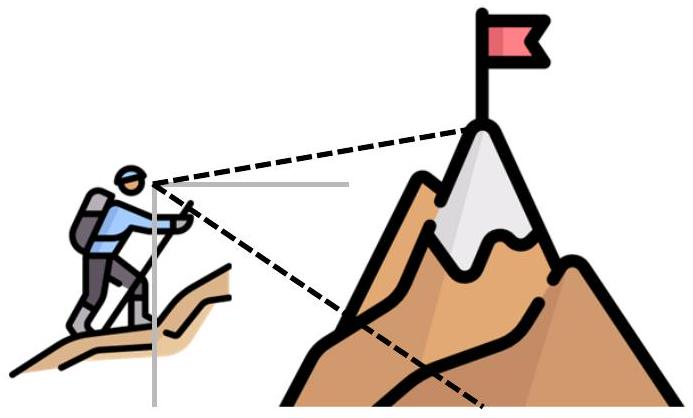
\includegraphics[max width=\textwidth, alt={}, center]{fb3a0175-091a-43c2-a0f1-82e1259502b5-03_418_693_397_1342}

Gina's phone can send and receive texts when she is within 45 miles of the cell phone tower. On a trip, Gina drives past the tower on Hwy 7 for 36 miles, and then she turns onto Oakville Road and drives for another 25 miles before stopping at Piggly Wiggly. Is Gina close enough to the transmission tower to be able to send and receive texts? Explain your reasoning.\\
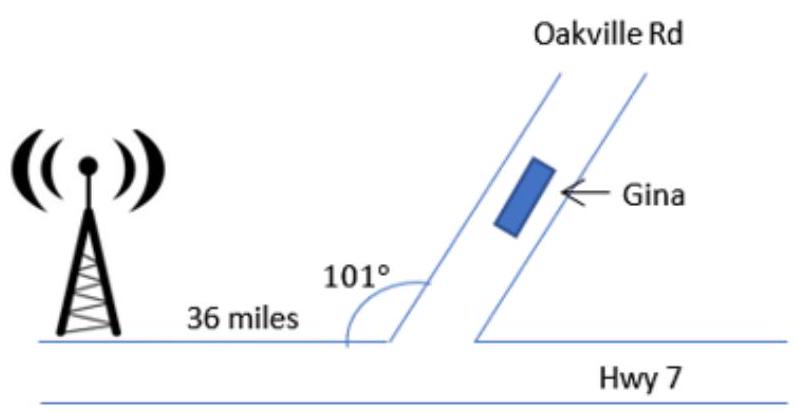
\includegraphics[max width=\textwidth, alt={}, center]{fb3a0175-091a-43c2-a0f1-82e1259502b5-03_412_798_1602_1173}

A ship full of monks leaves Port Sarim at 9:00 AM on Wednesday and heads towards Entrana. Entrana is located 700 miles at a bearing of $35^{\circ} \mathrm{E}$ of N from Port Sarim. To avoid a known kraken cove, the monks first head north for 12 hours at an average speed of 35 mph . Use this information to answer the following questions.\\
a) After traveling north for 12 hours, at what angle should they turn the boat to head directly to Entrana?\\
b) Assuming that they continue traveling at the same average speed, what time will they arrive on Entrana? Round your answer to the nearest minute.

A chicken and egg are in the middle of a heated argument. The chicken claims it is possible to create a triangle $A B C$, with side $A B$ measuring 24 inches, side $B C$ measuring 18 inches, and angle $A$ measuring $\frac{2 \pi}{9}$ radians. The egg claims this is not possible. Who is correct? Explain your reasoning.

\begin{enumerate}
  \item Find $B C$ in the triangle shown below. Round your answer to the nearest thousandth.
  \item Find $m \angle A$ in the triangle shown below. Round your answer to the nearest thousandth.
  \item A given triangle $A B C$ has $m \angle C=58^{\circ}, b=33, c=29$. Find all sides and angles of the triangle. Enter all possible answers if applicable. If no solutions exist, write "DNE" for all blanks and explain your reason. Show all necessary work. Round all answers to the nearest thousandth.\\
$a=$ $\_\_\_\_$\\
$b=$ $\_\_\_\_$\\
$c=$ $\_\_\_\_$\\
$m \angle A=$ $\_\_\_\_$\\
$m \angle B=$ $\_\_\_\_$\\
$m \angle C=$ $\_\_\_\_$
  \item A given triangle $A B C$ has $m \angle B=31^{\circ}, a=39, b=17$. Find all sides and angles of the triangle. Enter all possible answers if applicable. If no solutions exist, write "DNE" for all blanks and explain your reason. Show all necessary work. Round all answers to the nearest thousandth.\\
$a=$ $\_\_\_\_$\\
$b=$ $\_\_\_\_$\\
$c=$ $\_\_\_\_$\\
$m \angle A=$ $\_\_\_\_$\\
$m \angle B=$ $\_\_\_\_$\\
$m \angle C=$ $\_\_\_\_$
  \item A given triangle $A B C$ has $m \angle B=61^{\circ}, a=31, c=26$. Find all sides and angles of the triangle. Enter all possible answers if applicable. If no solutions exist, write "DNE" for all blanks and explain your reason. Show all necessary work. Round all answers to the nearest thousandth.\\
$a=$ $\_\_\_\_$\\
$b=$ $\_\_\_\_$\\
$c=$ $\_\_\_\_$\\
$m \angle A=$ $\_\_\_\_$\\
$m \angle B=$ $\_\_\_\_$\\
$m \angle C=$ $\_\_\_\_$
  \item A triangle has side lengths of 7, 9, and 11. Find the area of the triangle. Show all calculations that lead to your answer. Round your answer to the nearest thousandth.
\end{enumerate}

A rock climber is part of the way up a climb when he can see both the peak and the base of Gray Mountain. When viewing the peak of the mountain, his angle of elevation is $30^{\circ}$ above his eye level. When viewing the base of the mountain, his angle of depression is $41^{\circ}$ below his eye level. If he knows Gray Mountain is 3072 feet high and the base of the mountain is at sea level, then what is the elevation of the climber to the nearest inch?\\
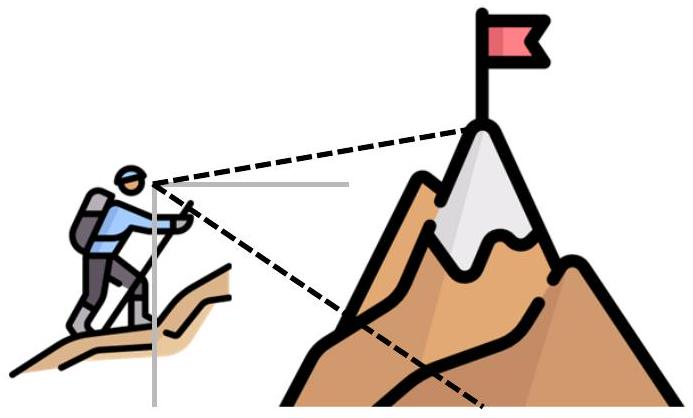
\includegraphics[max width=\textwidth, alt={}, center]{fb3a0175-091a-43c2-a0f1-82e1259502b5-07_418_693_397_1342}

Gina's phone can send and receive texts when she is within 50 miles of the cell phone tower. On a trip, Gina drives past the tower on Hwy 7 for 36 miles, and then she turns onto Oakville Road and drives for another 25 miles before stopping at Piggly Wiggly. Is Gina close enough to the transmission tower to be able to send and receive texts? Explain your reasoning.\\
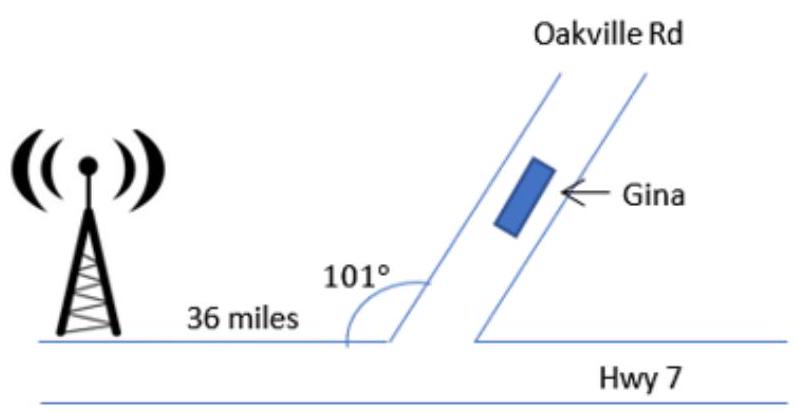
\includegraphics[max width=\textwidth, alt={}, center]{fb3a0175-091a-43c2-a0f1-82e1259502b5-07_412_798_1602_1173}

A ship full of monks leaves Port Sarim at 9:00 AM on Wednesday and heads towards Entrana. Entrana is located 650 miles at a bearing of $35^{\circ} \mathrm{N}$ of W from Port Sarim. To avoid a known kraken cove, the monks first head west for 12 hours at an average speed of 40 mph . Use this information to answer the following questions.\\
a) After traveling west for 12 hours, at what angle should they turn the boat to head directly to Entrana?\\
b) Assuming that they continue traveling at the same average speed, what time will they arrive on Entrana? Round your answer to the nearest minute.

A chicken and egg are in the middle of a heated argument. The chicken claims it is possible to create a triangle $A B C$, with side $A B$ measuring 24 inches, side $B C$ measuring 19 inches, and angle $A$ measuring $\frac{5 \pi}{18}$ radians. The egg claims this is not possible. Who is correct? Explain your reasoning.

\begin{enumerate}
  \item Find $B C$ in the triangle shown below. Round your answer to the nearest thousandth.
  \item Find $m \angle A$ in the triangle shown below. Round your answer to the nearest thousandth.
  \item A given triangle $A B C$ has $m \angle C=52^{\circ}, b=19, c=13$. Find all sides and angles of the triangle. Enter all possible answers if applicable. If no solutions exist, write "DNE" for all blanks and explain your reason. Show all necessary work. Round all answers to the nearest thousandth.\\
$a=$ $\_\_\_\_$\\
$b=$ $\_\_\_\_$\\
$c=$ $\_\_\_\_$\\
$m \angle A=$ $\_\_\_\_$\\
$m \angle B=$ $\_\_\_\_$\\
$m \angle C=$ $\_\_\_\_$
  \item A given triangle $A B C$ has $m \angle B=36^{\circ}, a=37, b=24$. Find all sides and angles of the triangle. Enter all possible answers if applicable. If no solutions exist, write "DNE" for all blanks and explain your reason. Show all necessary work. Round all answers to the nearest thousandth.\\
$a=$ $\_\_\_\_$\\
$b=$ $\_\_\_\_$\\
$c=$ $\_\_\_\_$\\
$m \angle A=$ $\_\_\_\_$\\
$m \angle B=$ $\_\_\_\_$\\
$m \angle C=$ $\_\_\_\_$
  \item A given triangle $A B C$ has $m \angle B=41^{\circ}, a=29, c=16$. Find all sides and angles of the triangle. Enter all possible answers if applicable. If no solutions exist, write "DNE" for all blanks and explain your reason. Show all necessary work. Round all answers to the nearest thousandth.\\
$a=$ $\_\_\_\_$\\
$b=$ $\_\_\_\_$\\
$c=$ $\_\_\_\_$\\
$m \angle A=$ $\_\_\_\_$\\
$m \angle B=$ $\_\_\_\_$\\
$m \angle C=$ $\_\_\_\_$
  \item A triangle has side lengths of 7, 11, and 14. Find the area of the triangle. Show all calculations that lead to your answer. Round your answer to the nearest thousandth.
\end{enumerate}

A rock climber is part of the way up a climb when he can see both the peak and the base of Gray Mountain. When viewing the peak of the mountain, his angle of elevation is $31^{\circ}$ above his eye level. When viewing the base of the mountain, his angle of depression is $38^{\circ}$ below his eye level. If he knows Gray Mountain is 4081 feet high and the base of the mountain is at sea level, then what is the elevation of the climber to the nearest inch?\\
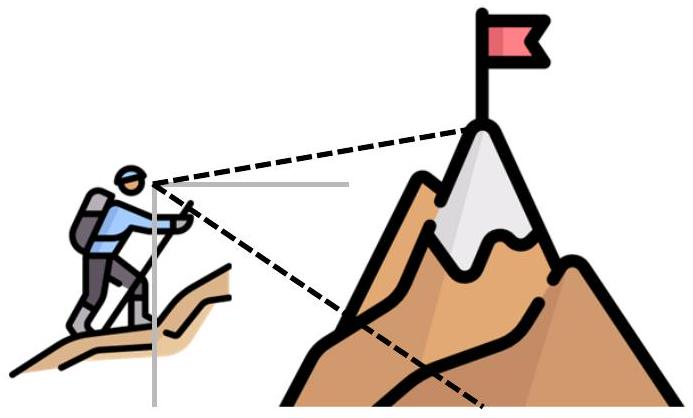
\includegraphics[max width=\textwidth, alt={}, center]{fb3a0175-091a-43c2-a0f1-82e1259502b5-11_418_693_397_1342}

Gina's phone can send and receive texts when she is within 50 miles of the cell phone tower. On a trip, Gina drives past the tower on Hwy 7 for 36 miles, and then she turns onto Oakville Road and drives for another 30 miles before stopping at Piggly Wiggly. Is Gina close enough to the transmission tower to be able to send and receive texts? Explain your reasoning.\\
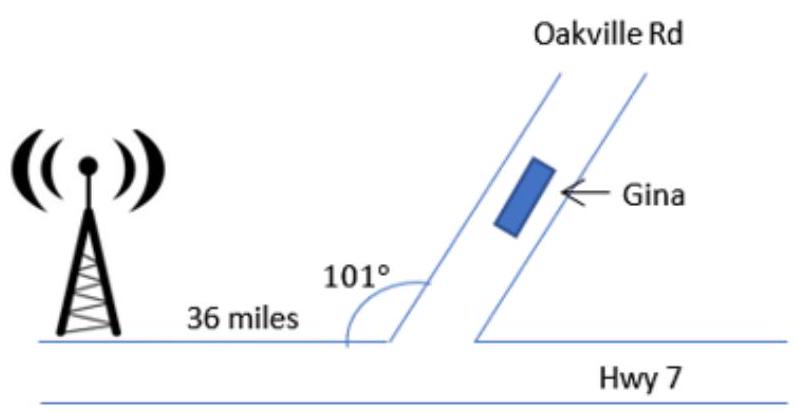
\includegraphics[max width=\textwidth, alt={}, center]{fb3a0175-091a-43c2-a0f1-82e1259502b5-11_412_798_1602_1173}

A ship full of monks leaves Port Sarim at 9:00 AM on Wednesday and heads towards Entrana. Entrana is located 750 miles at a bearing of $35^{\circ} \mathrm{W}$ of N from Port Sarim. To avoid a known kraken cove, the monks first head north for 10 hours at an average speed of 40 mph . Use this information to answer the following questions.\\
a) After traveling north for 10 hours, at what angle should they turn the boat to head directly to Entrana?\\
b) Assuming that they continue traveling at the same average speed, what time will they arrive on Entrana? Round your answer to the nearest minute.

A chicken and egg are in the middle of a heated argument. The chicken claims it is possible to create a triangle $A B C$, with side $A B$ measuring 31 inches, side $B C$ measuring 18 inches, and angle $A$ measuring $\frac{\pi}{5}$ radians. The egg claims this is not possible. Who is correct? Explain your reasoning.


\end{document}